\documentclass{beamer}
\usetheme{ttuStatsCamp}
\usefonttheme{serif}
\usepackage[T1]{fontenc}
\usepackage[utf8]{inputenc}
%\usepackage{mathptmx}
\usepackage{url}
\usepackage{graphicx}
\usepackage{setspace}
%\usepackage{esint}
\usepackage[natbibapa]{apacite}
\usepackage{color}
\usepackage{amsmath}
\usepackage{amsfonts}
%\usepackage{bm}
\usepackage{Sweavel}
\usepackage{listings}

\def\Sweavesize{\scriptsize}
\def\Rcolor{\color{black}}
%\def\Routcolor{\color{red}}
\def\Rcommentcolor{\color{violet}}
\def\Rbackground{\color[gray]{0.85}}
\def\Routbackground{\color[gray]{0.85}}

\lstset{tabsize=2, breaklines=true, style=Rstyle}



\newcommand{\red}[0]{\textcolor{red}}
%\newcommand{\violet}[0]{\textcolor{violet}}
\newcommand{\green}[0]{\textcolor{green}}
\newcommand{\blue}[0]{\textcolor{blue}}
\newcommand{\comment}[1]{}
\newcommand{\kfold}[0]{\emph{K}-fold cross-validation}
\newcommand{\va}[0]{\vspace{12pt}}
\newcommand{\vb}[0]{\vspace{6pt}}
\newcommand{\vc}[0]{\vspace{3pt}}
\newcommand{\vx}[1]{\vspace{#1pt}}
\newcommand{\lang}[1]{\textsf{#1}}
\newcommand{\pkg}[1]{\textbf{#1}}

\title[Lecture 1]{Lecture 1: Introduction}

\author{Kyle M. Lang}

\institute[TTU IMMAP]{
  Institute for Measurement, Methodology, Analysis \& Policy\\
  Texas Tech University\\
  Lubbock, TX
}

\date{2016 Stats Camp}


\begin{document}

\setkeys{Gin}{width=\textwidth}

\input{sweaveFiles/-001}


\begin{frame}[plain]
  
  \titlepage
  
\end{frame}


\begin{frame}{Personal Introductions}
  
  Please give the following information:
  \vb
  \begin{enumerate}
    \item Name
      \vb
    \item Home-base
      \vb
    \item Prior experience with linear regression
      \vb
    \item Prior experience with structural equation modeling
      \vb
    \item Prior experience with \textsf{R}
      \vb
    \item Interest in this course
      \vb
    \item Favorite animal with a name beginning with the letter \emph{B}
  \end{enumerate}
  
\end{frame}


\begin{frame}{Outline}

  \begin{itemize}
  \item Framing mediation, moderation, and conditional process analysis
    \va
  \item Rough outline of what we'll cover this week
    \va
  \item Get everyone up and running with \textsf{R}
  \end{itemize}

\end{frame}


\begin{frame}{General Context}
  
  What do we mean by \emph{mediation} and \emph{moderation}?\\  
  \pause
  \va
  Mediation and moderation are types of hypotheses, not statistical
  methods or models.
  \begin{itemize}
  \item Mediation tells us \emph{how} one variable influences another.
    \vb
  \item Moderation tells us \emph{when} one variable influences another.
  \end{itemize}
    
\end{frame}


\begin{frame}{Contextualizing Example}
  
  Say we wish to explore the process underlying exercise habits.\\
  \va
  Our first task is to operationalize ``exercise habits''
  \begin{itemize}
    \item DV: Hours per week spent in vigorous exercise
      (\emph{exerciseAmount}).
  \end{itemize}
  \va 
  We may initial ask: what predicts devoting more time to
  exercise?
  \begin{itemize}
    \item IV: Concerns about negative health outcomes
      (\emph{healthConcerns}).
  \end{itemize}
 
\end{frame}


\begin{frame}{Focal Effect Only}
  
  The $healthConcerns \rightarrow exerciseAmount$ relation is our
  \emph{focal effect}
  
  \vx{-48}
  
  \begin{figure}
    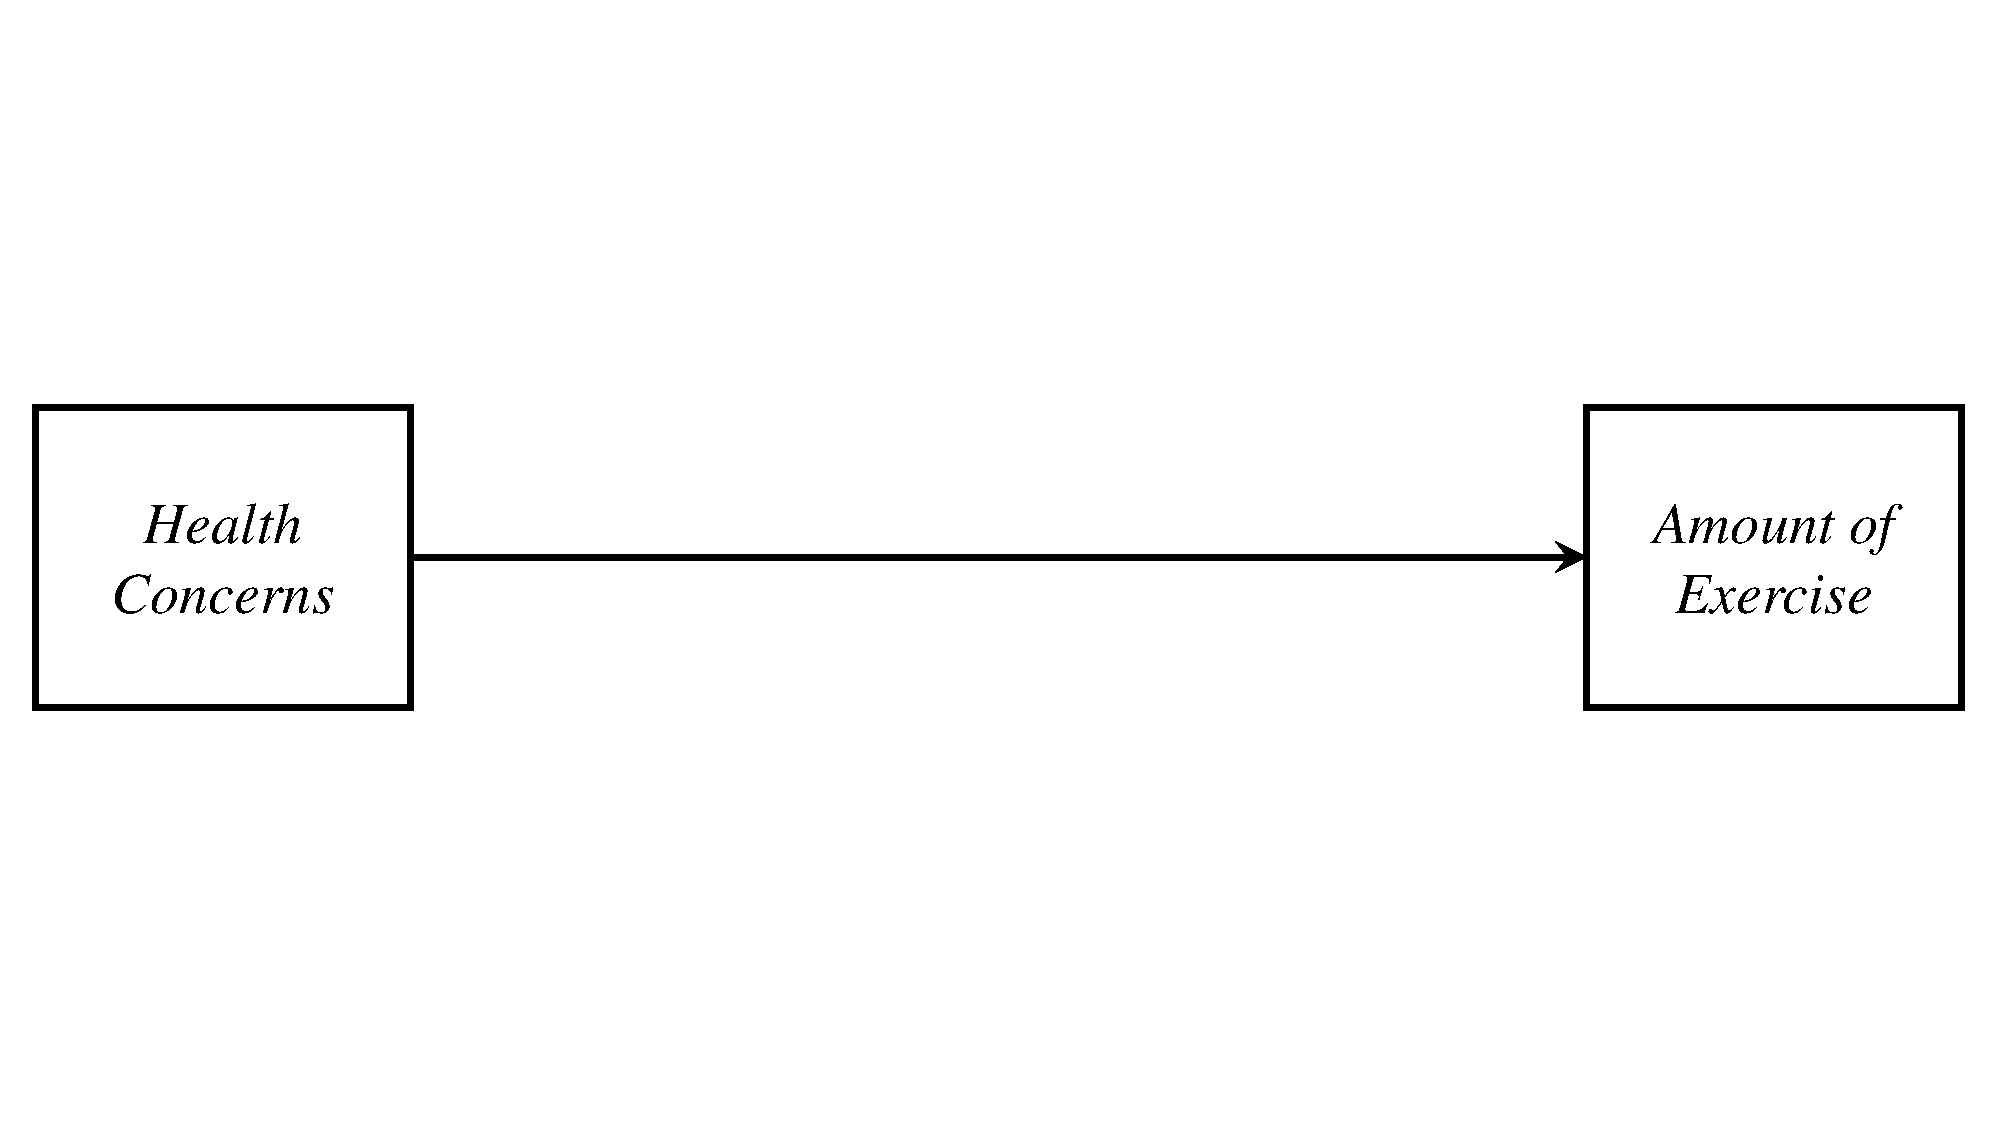
\includegraphics[width=\textwidth]{figures/focalEffectDiagram.pdf}
  \end{figure}
 
  \vx{-48}
  
   \begin{itemize}
    \item Mediation, moderation, and conditional process analysis all
      attempt to describe the focal effect in more detail.
      \vb
    \item We always begin by hypothesizing a focal effect.
  \end{itemize}
 
\end{frame}



\begin{frame}{The Mediation Hypothesis}

  A mediation analysis will attempt to describe how health concerns
  affect amount of exercise.
  \va
  \begin{itemize}
  \item The \emph{how} is operationalized in terms of intermediary
    variables.
    \va
  \item Mediator: Motivation to improve health (\emph{motivation}).
  \end{itemize}
  
  \vx{-18}

  \begin{figure}
    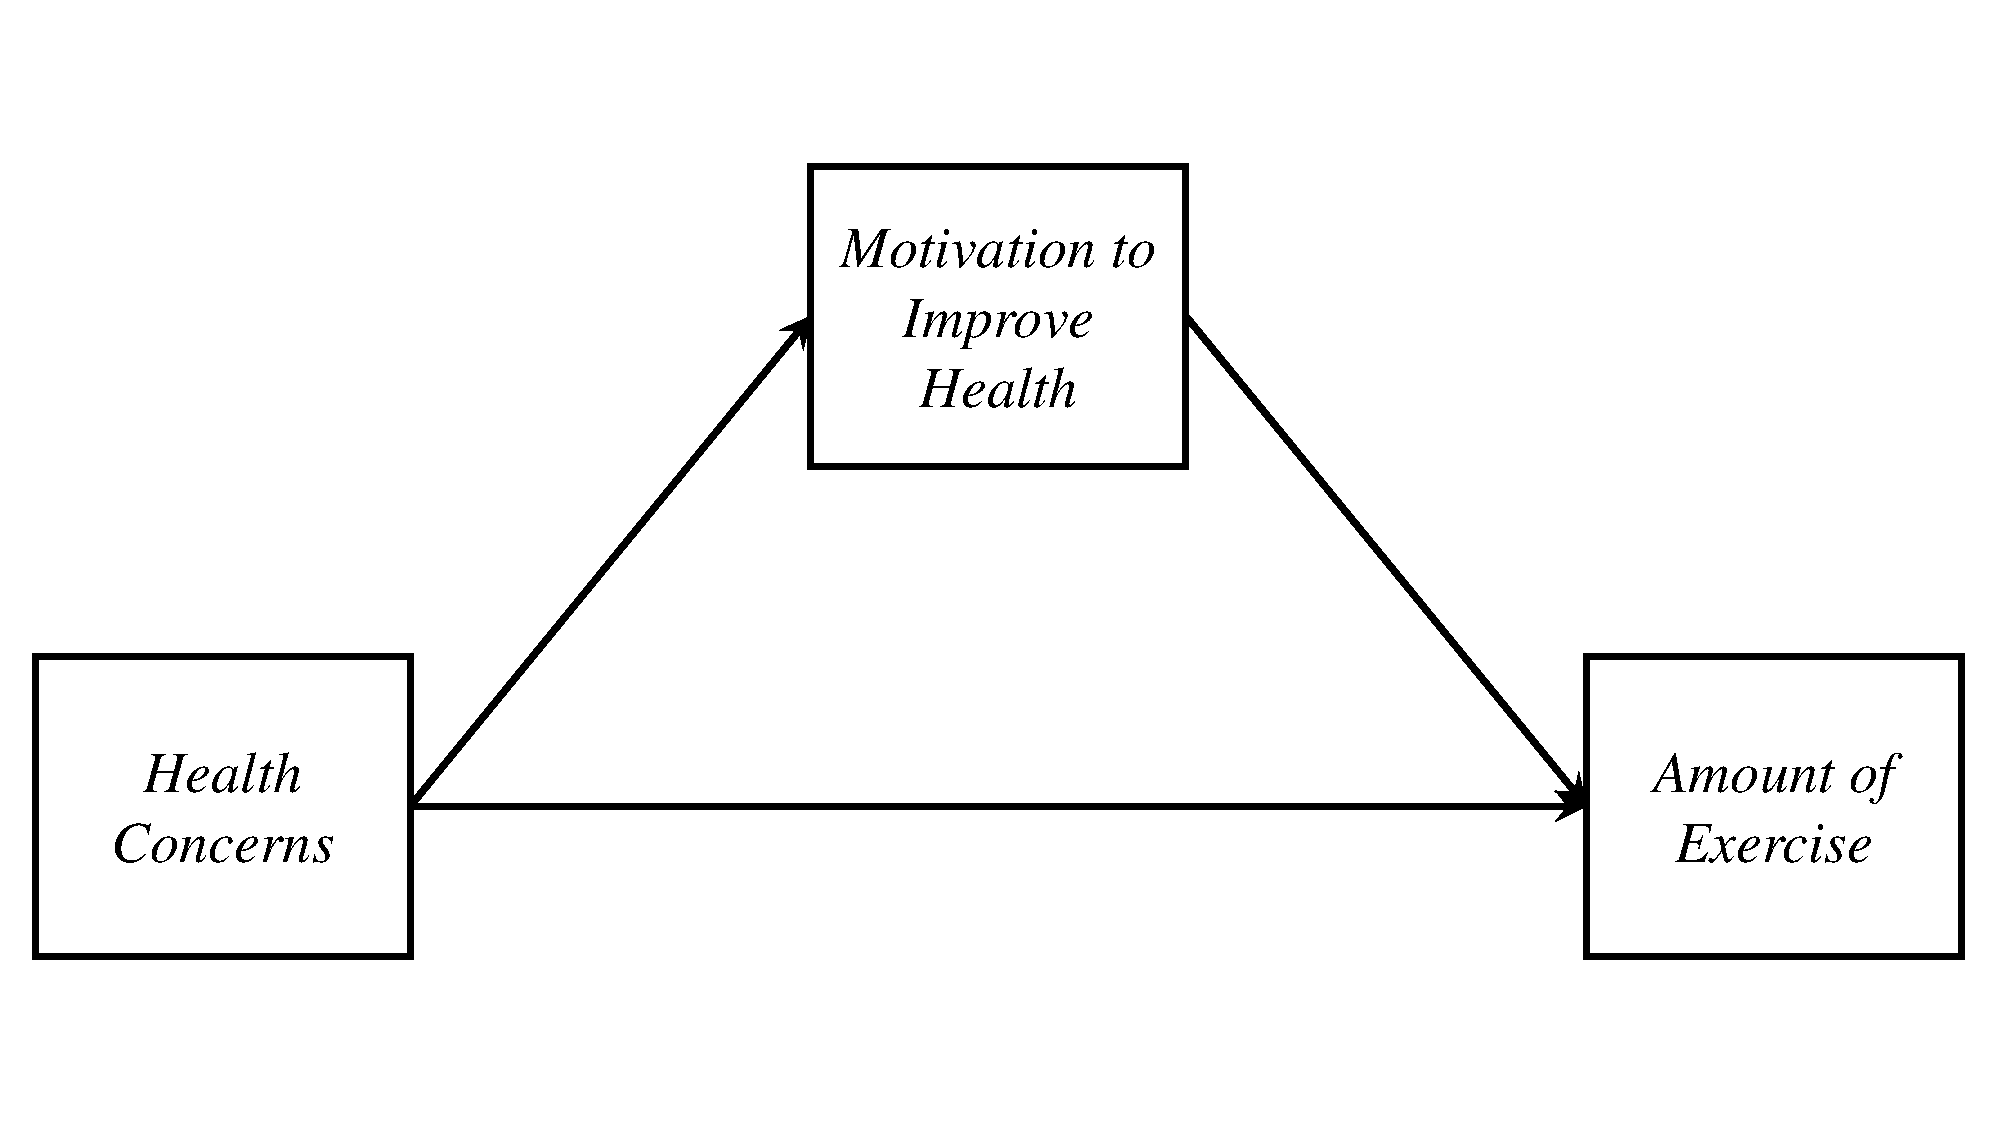
\includegraphics[width=.8\textwidth]{figures/mediationDiagram.pdf}
  \end{figure}
  
\end{frame}


\begin{frame}{Moderation Hypothesis}
  
  A moderation hypothesis will attempt to describe when health
  concerns affect amount of exercise.
  \va
  \begin{itemize}
    \item The \emph{when} is operationalized in terms of interactions
      between the focal predictor and contextualizing variables
      \va
    \item Moderator: Sense of personal agency relating to physical
      health (\emph{agency}).
  \end{itemize}

  \vx{-18}
  
  \begin{figure}
    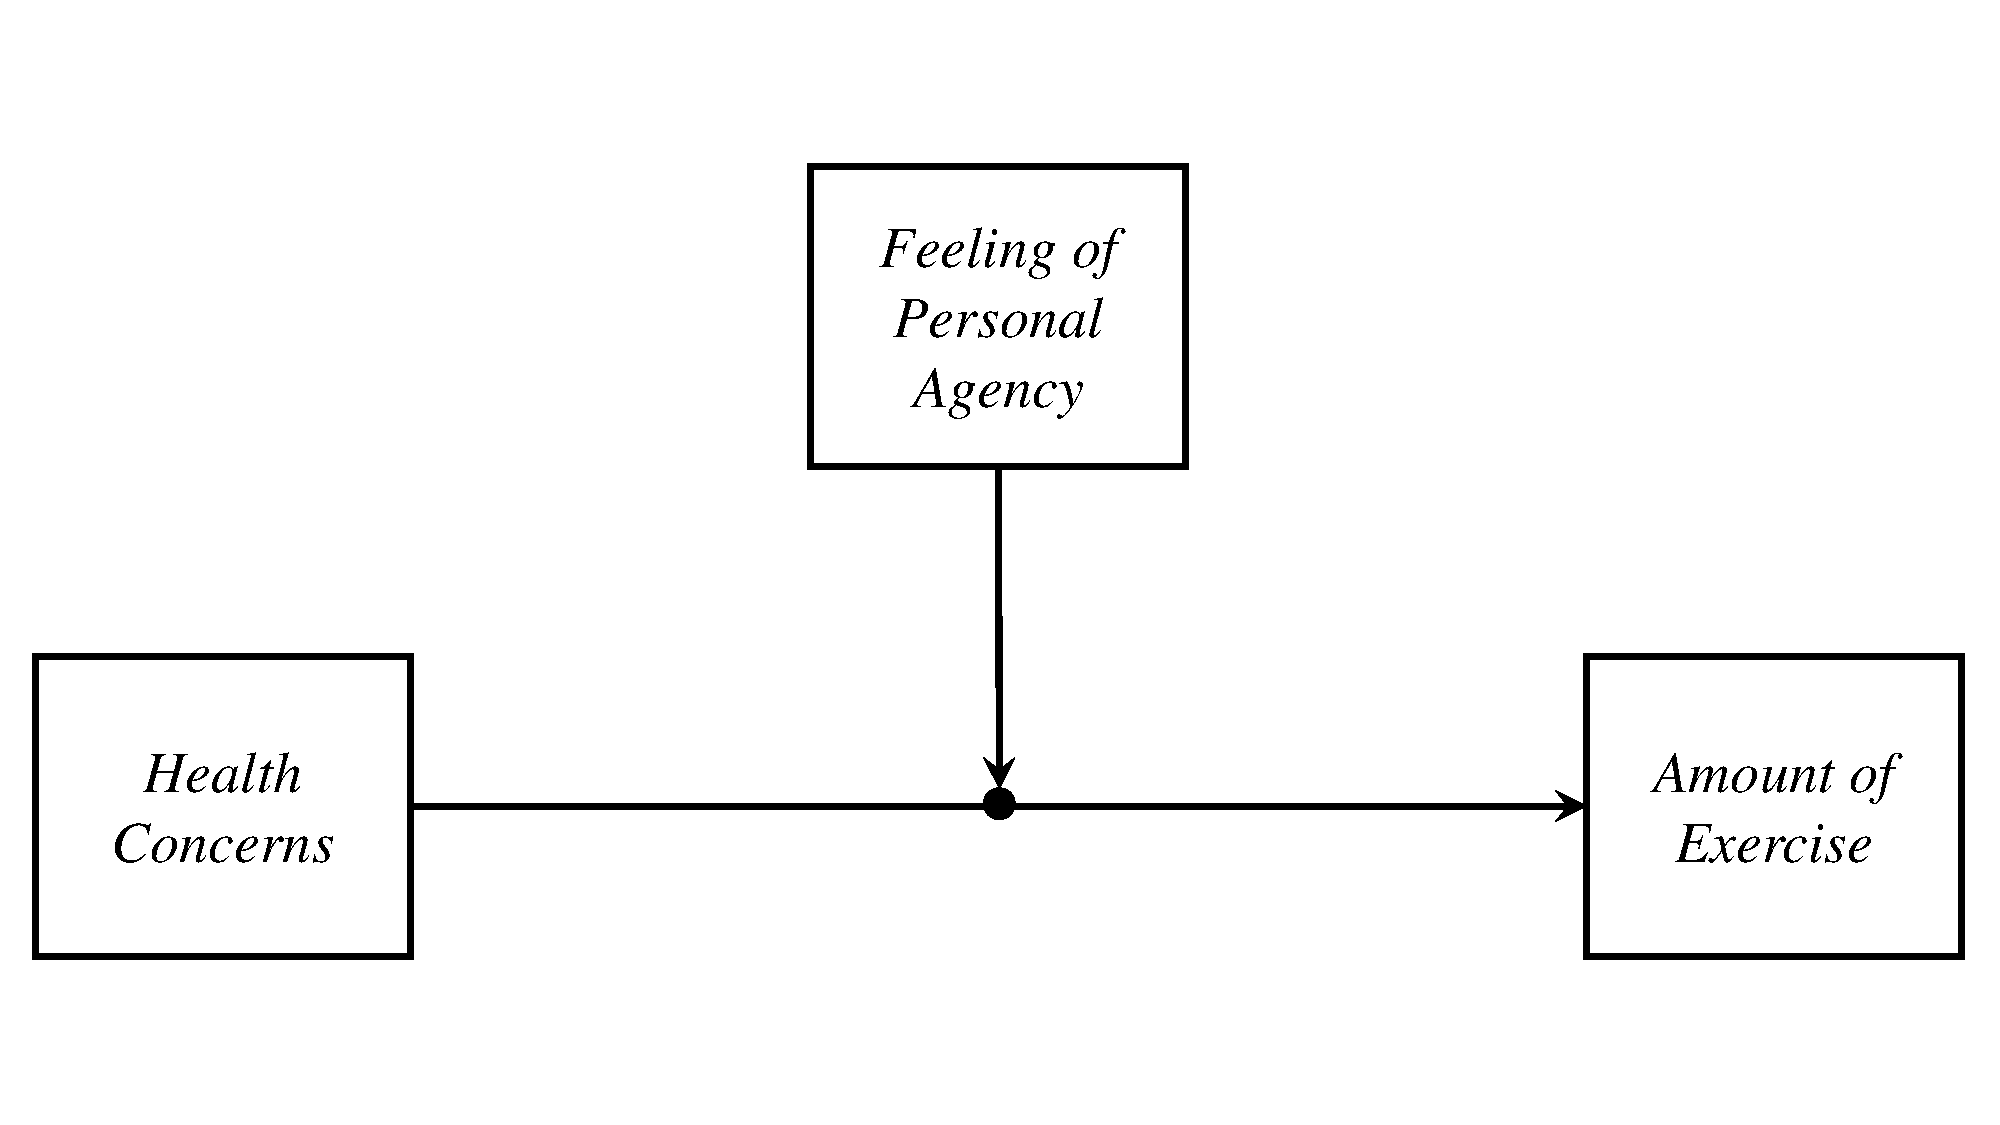
\includegraphics[width=.8\textwidth]{figures/moderationDiagram.pdf}
  \end{figure}
  
\end{frame}


\begin{frame}{Conditional Process Analysis}
  
  Conditional process analysis combines the mediation and moderation
  hypotheses into models of moderated mediation.
  \va
  \begin{itemize}
    \item Given a mediation model describing \emph{how} health
      concerns affect exercise amount, what other variables may
      modulate the indirect effect.
  \end{itemize}
  
\end{frame}

\begin{frame}{}
  
  \begin{center}\huge{\textsc{Software Setup Time!}} \end{center}
  
\end{frame}


\begin{frame}{What is \lang{R}?}
  
  \lang{R} is a holistic (open-source) software system for data
  analysis and statistical programming.  
  \vb
  \begin{itemize}
  \item Introduced by \citet{ihakaGentleman:1996} and currently
    maintained by a core group of statistical programmers known as
    the \emph{R Core Team}.
    \vb
  \item Support by thousands of world-wide contributors.  \vc
    \begin{itemize}
      \item Anyone can contribute an R package to the
        \emph{Comprehensive R Archive Network} (CRAN) if it conforms
        to the licensing and formatting/packaging requirements of the
        R-Project.
    \end{itemize}
    \vb
  \item Considered a dialect/implementation of the \lang{S} language
    developed by John Chambers \citep{beckerChambers:1984,
      beckerEtAl:1988, chambersHastie:1992, chambers:1998}.
  \end{itemize}
  
\end{frame}


\begin{frame}{What is \lang{R}?}
  
  I prefer to think about \lang{R} as a \emph{statistical programming
    language}, rather than as a data analysis program.
  \vb
  \begin{itemize}
  \item \lang{R} \textbf{IS NOT} its GUI (no matter which GUI you use).
    \vb
  \item You can write \lang{R} code in whatever program you like
    (e.g., RStudio, EMACS, Notepad, directly in the
    console/shell/command line).
    \vb
  \item R can be used for basic (or advanced) data analysis, but its
    real strength is its flexible programming framework.
    \vc
    \begin{itemize}
      \item Tedious tasks can be automated.
        \vc
      \item Computationally demanding jobs can be run in parallel.
        \vc
      \item \lang{R}-based research \emph{wants} to be reproducible.
        \vc
      \item Analyses are automatically documented via their scripts.
    \end{itemize}
  \end{itemize}
  
\end{frame}


\begin{frame}{Getting \lang{R}}
  
  \lang{R} can be downloaded, for free, from the following webpage:
  \va
  \begin{itemize}
  \item \url{https://www.r-project.org/}
  \end{itemize}
  \va 
  You will also need a proper text editor. For those who are just
  learning \lang{R}, I recommend \pkg{RStudio}: 
  \va
  \begin{itemize}
  \item \url{https://www.rstudio.com/}
  \end{itemize}
  
\end{frame}

      
\begin{frame}[allowframebreaks]{References}
  \bibliographystyle{apacite}
  \bibliography{../../bibtexStuff/rRefs.bib}
\end{frame}

\end{document}
